% $Header: quali_main.tex $

%\setbeamertemplate{footline}[page number]
\setbeamertemplate{footline}[frame number]

\mode<presentation>
{
%  \usepackage[orientation=landscape,size=custom,width=15,height=9,scale=0.5,debug]{beamerposter} 
  \usepackage[orientation=landscape,size=custom,width=12,height=9,scale=0.49,debug]{beamerposter} 

  \usepackage{lmodern}
  \usepackage{fix-cm}

  \setbeamertemplate{blocks}[rounded][shadow=true]
  \usetheme{BeloHorizonte}
  % \usetheme{Madrid}
  
  \setbeamercovered{transparent}
  
  %% pula meia linha entre parágrafos
  \addtolength{\parskip}{0.5\baselineskip}
%  \setlength{\topsep}{-10.0mm}
  \setlength{\partopsep}{-0.6\partopsep}

  
  \usepackage{mathptmx}
  \usepackage{pgf}
  
  \def\newblock{}
  \usepackage{natbib}
}

% \AtBeginSection[]{  \begin{frame*}<beamer>    \setlength{\parskip}{0pt}    \frametitle{Sumário}    \tableofcontents[currentsection]  \end{frame*}}

\usepackage{appendixnumberbeamer}
\usepackage{xspace}
\usepackage{multirow}
\usepackage{colortbl}
\usepackage{rotating}  %% p usar vertical, escrever tombado
\usepackage{booktabs}
\usepackage{tabularx}
\usepackage{amsmath}
\usepackage[absolute,overlay]{textpos}
\usepackage{tcolorbox}

%\usepackage{hyperref}


%% tabular x stuff
\newcolumntype{C}{>{\centering\arraybackslash}X}%
\newcolumntype{R}{>{\raggedleft\arraybackslash}X}%

\usepackage[portuguese,english]{babel}

\usepackage{ucs}
\usepackage[utf8x]{inputenc}
\usepackage[T1]{fontenc} %% Generate proper accented word on the PDF output, so
                         %% you can copy-paste from it.

%\usepackage{sfmath}

\usepackage{rotate}
\usepackage{graphicx}
\usepackage{subfigure}

%\def\newblock{\hskip .11em plus .33em minus .07em}
\usepackage{url}


\usepackage{float}
\restylefloat{figure}

\usepackage{calc}
\usepackage[center]{caption}


\graphicspath{{./figures/}}


%% Arruma estilão do sumário
%\usepackage{tocloft}
\usepackage{setspace}

\renewcommand{\thefootnote}{\fnsymbol{footnote}}



%%%%%%%%%%%%%%%%%%%%%%%%%%%%%%%%%%%%%%%%%%%%%%%%%%%%%%%%%%%
%%%%%%%%%%%%%%%%%%%%%%%%%%%%%%%%%%%%%%%%%%%%%%%%%%%%%%%%%%%
%%%
%%%
\title[Defesa de doutorado]{Corisco: Robust edgel-based orientation estimation for\\ generic camera models}

\author[N. Werneck]{Nicolau~L.~Werneck\\
\usebox{\myurl}
}


\institute[LTI---PCS---USP]
{ Supervisor: { Profa. Dra. Anna Helena Reali Costa}\\
  Intelligent Techniques Laboratory, LTI --- PCS --- Poli\\
  \large Universidade de São Paulo}

\date{Augsburg, Deutschland --- 8/10/2015}

%\beamerdefaultoverlayspecification{<+->}


\newcommand{\corisco}{{\sl Corisco}\xspace}

\newcommand{\tee}{\mathrm{t}}
\newcommand{\sen}{\mathrm{sen}}
\newcommand{\vP}{{\boldsymbol{\Psi}}}
\newcommand{\Pa}{{\Psi^a}}
\newcommand{\Pb}{{\Psi^b}}
\newcommand{\Pc}{{\Psi^c}}
\newcommand{\Pd}{{\Psi^d}}
\newcommand{\vK}{{\mathbf{K}}}

\newcommand{\vv}{{\mathbf{v}}}
\newcommand{\vu}{{\mathbf{u}}}
\newcommand{\vr}{{\mathbf{r}}}
\newcommand{\vp}{{\mathbf{p}}}
\newcommand{\vn}{{\mathbf{n}}}
\newcommand{\vq}{{\mathbf{q}}}
\newcommand{\vx}{{\mathbf{x}}}
\newcommand{\vJ}{{\mathbf{J}}}

\newcommand{\vc}{{\mathbf{c}}}
\newcommand{\vd}{{\mathbf{d}}}
\newcommand{\vdd}{{\mathbf{d}^\prime}}
\newcommand{\vg}{{\mathbf{g}}}
\newcommand{\vH}{{\mathbf{H}}}
\newcommand{\vI}{{\mathbf{I}}}
\newcommand{\vA}{{\mathbf{A}}}
\newcommand{\vZ}{{\mathbf{Z}}}
\newcommand{\vS}{{\mathbf{S}}}
\newcommand{\vy}{{\mathbf{y}}}
\newcommand{\vyy}{{\mathbf{y}^\prime}}
\newcommand{\vb}{{\mathbf{b}}}
\newcommand{\vbb}{{\mathbf{b}^\prime}}
\newcommand{\vM}{{\mathbf{M}}}
\newcommand{\vm}{{\mathbf{m}}}
\newcommand{\vw}{{\mathbf{w}}}

\newcommand{\vmu}{\mu_{1\cdots K}}




%%%
%%%
%%%
\begin{document}


%%
\begin{frame}[plain]
  \titlepage
\end{frame}
\addtocounter{framenumber}{-1}

% %%
% \begin{frame}{Sumário}
% \setlength{\parskip}{0pt}
% \tableofcontents
% \end{frame}



%%%%%%%%%%%%%%%%%%%%%%%%%%%%%%
%%%%%%%%%%%%%%%%%%%%%%%%%%%%%%
\section[1--Introdução]{Introduction}

%%
%%
\begin{frame}{Meta-introduction}
Nicolau Werneck, Sc.D.
\begin{itemize}
\item E.Eng. graduated from UFMG, Unicamp and USP.
\item Specialized in signal processing and pattern recognition, especially in computer vision and parameter estimation problems.
\item Ex-Google and ex-Geekie.
\item Wants to help robots help us.
\end{itemize}

Presentation adapted from my doctorate defense. Results were published in~\citet{Werneck2013}.

\end{frame}


%%
%%
\begin{frame}{Presentation Schedule}
  \begin{enumerate}
  \item Problem introduction
  \item How \corisco works
  \item Experiments
  \item Conclusion
  \end{enumerate}
\end{frame}



%%
%%
\begin{frame}{Anthropic Environments}


An {\em anthropic environment} is composed by straight lines, parallel to the directions of a {\em natural reference frame}.
  
The orientation we find is a three-dimensional rotation between the natural and the camera reference frame.

  \hspace{0.0\baselineskip}\centerline{
    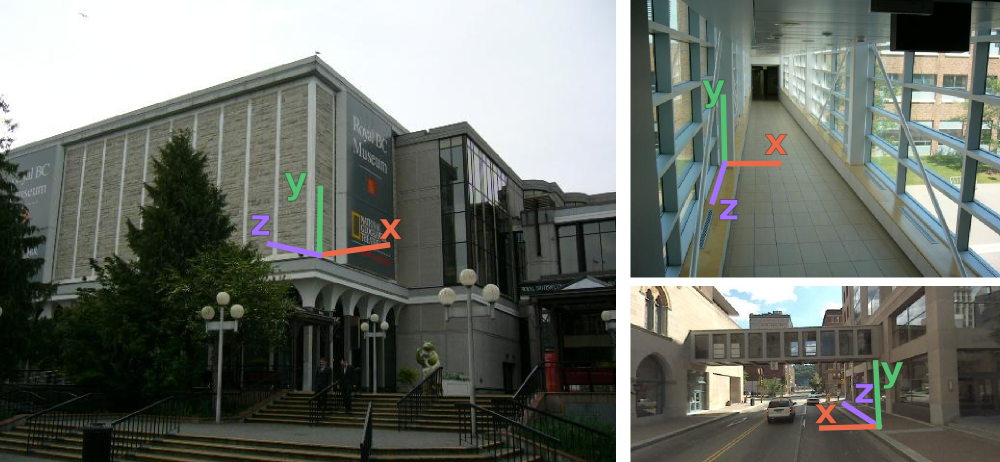
\includegraphics[height=9\baselineskip]{antrop.png}
  }
\end{frame}


%%
%%
\begin{frame}{Edgels and straight lines}
  Edgels are points samples over curves or (straight) lines.
  \centerline{
    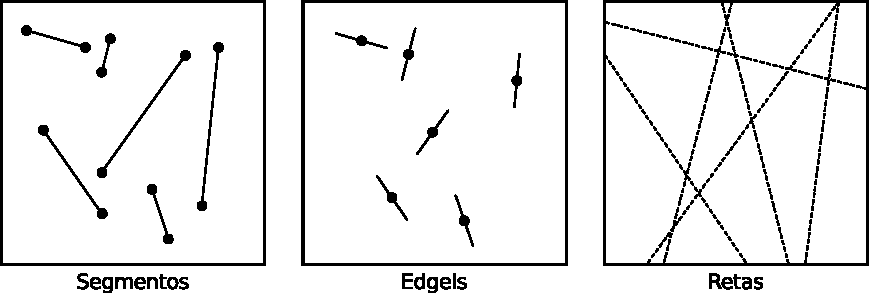
\includegraphics[height=5\baselineskip]{lineseg.pdf}
  }
  
  Edgels have many applications.
  \centerline{
    \includegraphics[height=5.5\baselineskip]{snake_example.jpg}\quad
    \includegraphics[height=5.5\baselineskip]{eade_edge.jpg}
  }
\end{frame}


%%
%%
\begin{frame}{Proposal}
  \begin{overprint}
    \alert<+>{} We proposed a \alert<+>{monocular} vision method,
    denominated \corisco, that can estimate the orientation of a camera relative to an anthropic environment.\alert<+>{}

    Evolution of existing edgel based methods \citep{Coughlan2003}.

    Aplication examples:\\
    \begin{itemize}
    \item Guiding a mobile robot.
    \item Initial estimates for multi-view reconstruction.
    \item Object orientation estimation.
    \end{itemize}
  \end{overprint}
\end{frame}


%%
%%
\begin{frame}{Contributions}
  \corisco has the following peculiarities:\\
  \begin{itemize}
  \item Supports any possible camera model.
  \item Compromise between speed and precision.
  \item No assumptions about the solution.
  \item Dismisses the use of very costly operations ({\tt sin}, {\tt atan},
    {\tt exp}, {\tt log}). Uses the function $x^{-1/2}$.
  \end{itemize}
\end{frame}


%%
%%
\begin{frame}{High-level view}{}
  {\bf Inputs:} Image, control and intrinsic parameters.\\
  {\bf Output:} Orientation $\vP$ (three-dimensional rotation).
  \vfill
  \centerline{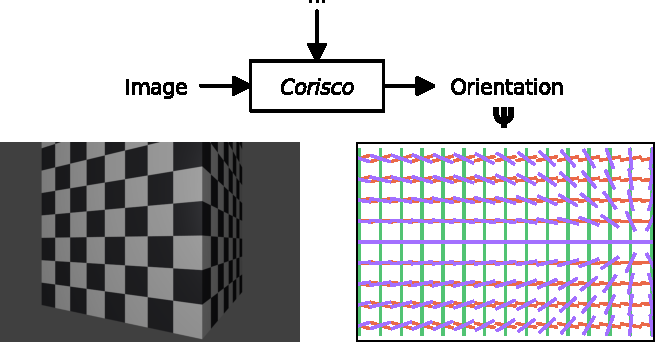
\includegraphics[height=11\baselineskip]{cg.pdf}}    
  \end{frame}


%%
%%
\begin{frame}{Geometria}
  A direção $\vv$ de uma reta sobre o ponto $\vp$ depende de $\vP$.
  \[
  (\vP,\vp) \rightarrow \vv
  \]

  \centerline{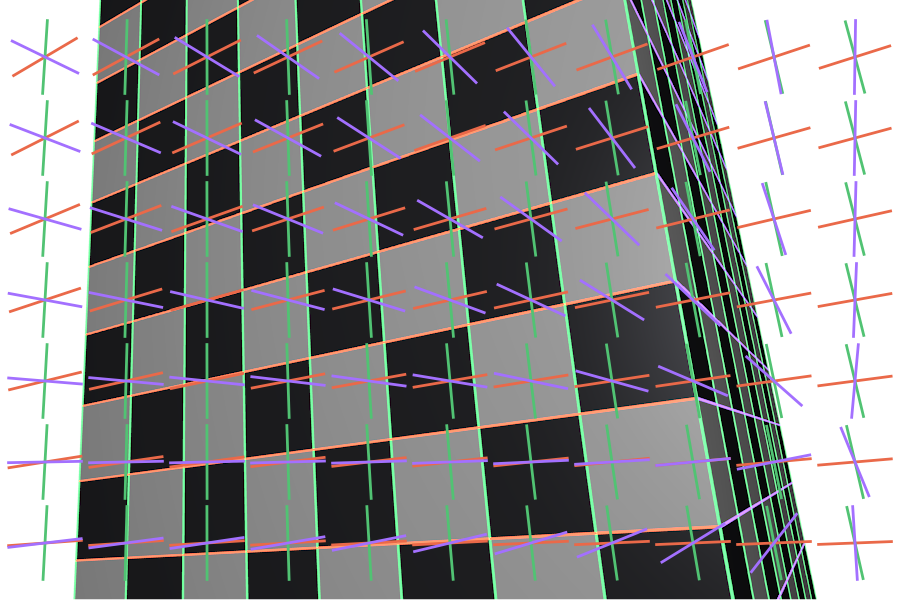
\includegraphics[height=10\baselineskip]{canim0117.png}}

  \hfill\raisebox{\baselineskip}{\textcolor{black!20}{\scriptsize\url{http://youtu.be/PbUyvdnBIzs}}}
\end{frame}



%%%%%%%%%%%%%%%%%%%%%%%%%%%%%%
%%%%%%%%%%%%%%%%%%%%%%%%%%%%%%
%%
%%
\begin{frame}{Objetivo}
  \begin{block}{Nossa pergunta}
    {\em Qual seria a melhor forma de estimar a orientação de câmera em
      \alert<2>{tempo real} em um ambiente antrópico a partir de uma única
      \alert<2>{imagem distorcida}?}
  \end{block}
\end{frame}


\begin{frame}{Edgels {\em versus} retas}
  A orientação pode ser encontrada por retas
  (\cite{Caprile1990,Cipolla1999,Rother2002}).\\ %Cipolla1999,Rother2002
  \begin{itemize}
  \item Mais intuitivos.
  \item Alcançam boas precisões.
  \end{itemize}

 No entanto:\\
  \begin{itemize}
  \item Restrição à projeção perspectiva.
  \item Complexidade da extração de retas.%\\(Número indeterminado de classes.)
  \end{itemize}

  Edgels permitem lidar com distorções e são mais fáceis de extrair e de sub-amostrar.
\end{frame}


%%
%%
\begin{frame}{Detalhamento do Corisco}
  \only<+>{\centerline{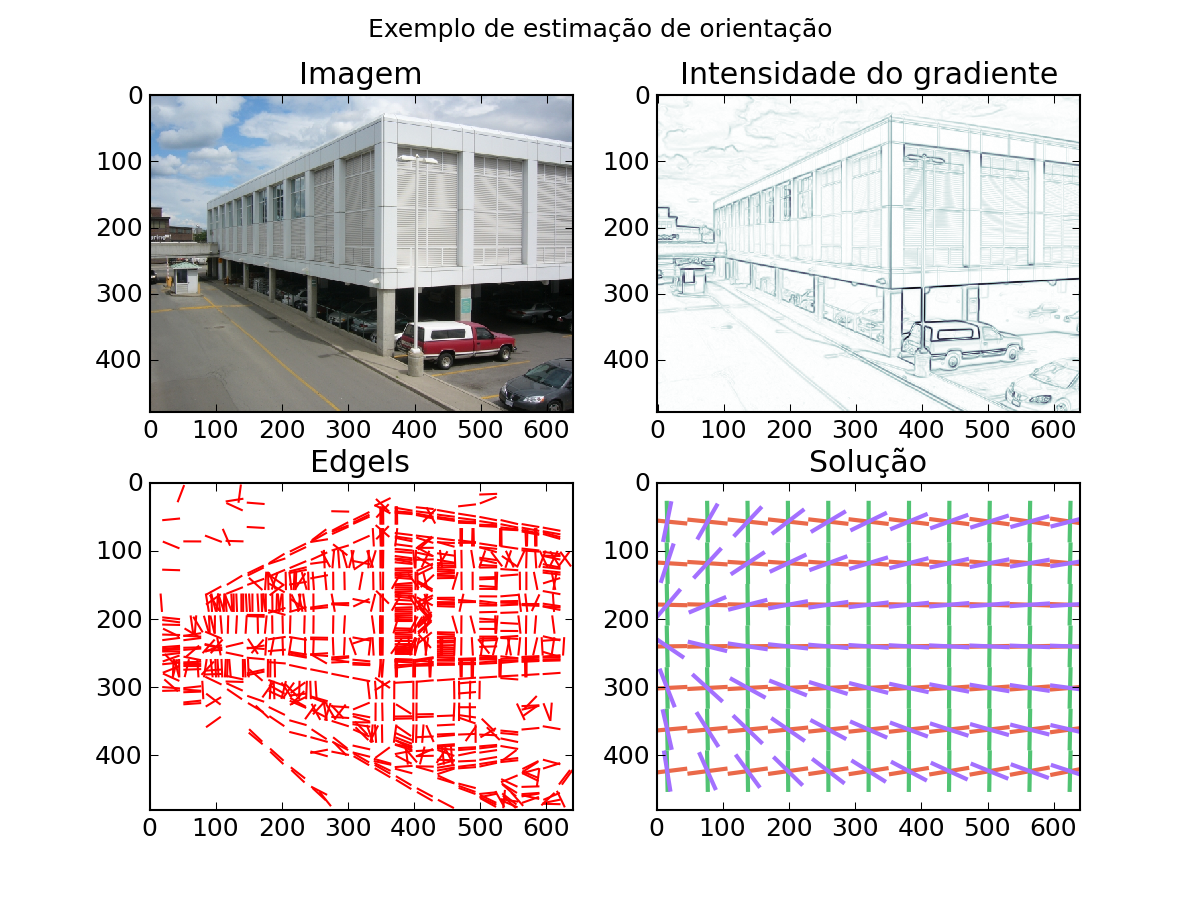
\includegraphics[height=14.2\baselineskip]{oriex91.png}}}
  \only<+>{\centerline{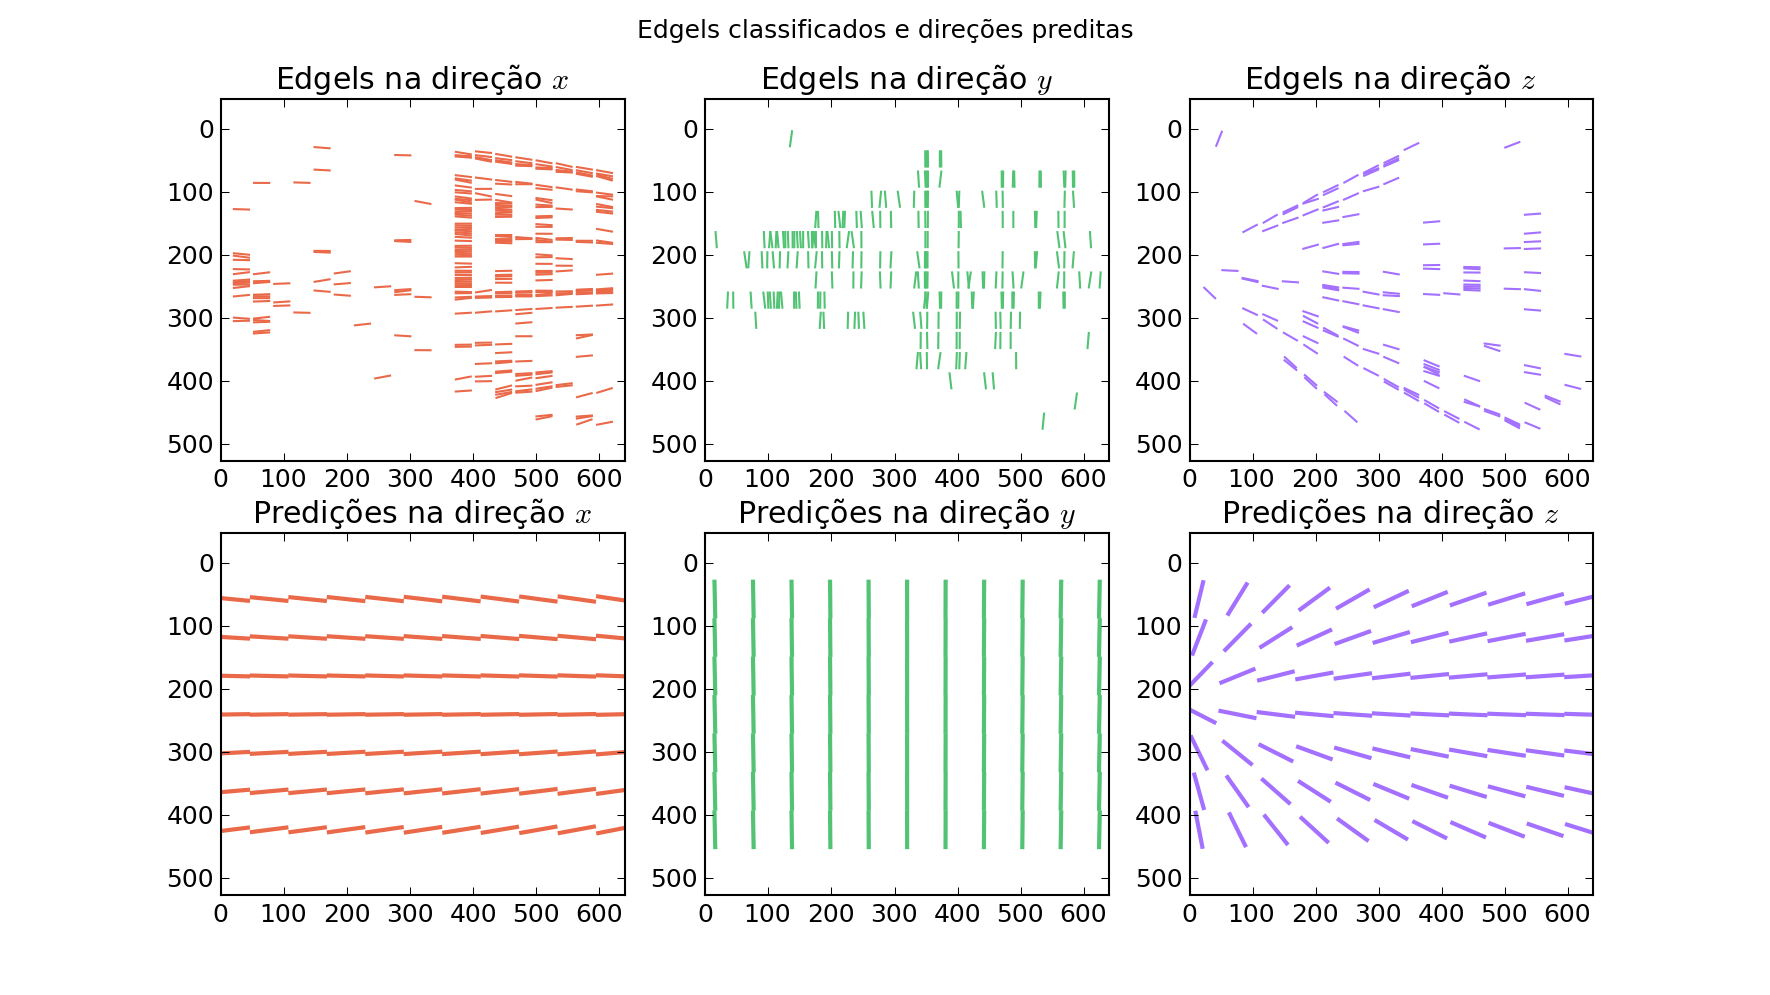
\includegraphics[height=14.2\baselineskip]{sep_york91.png}}}
  \only<+>{\centerline{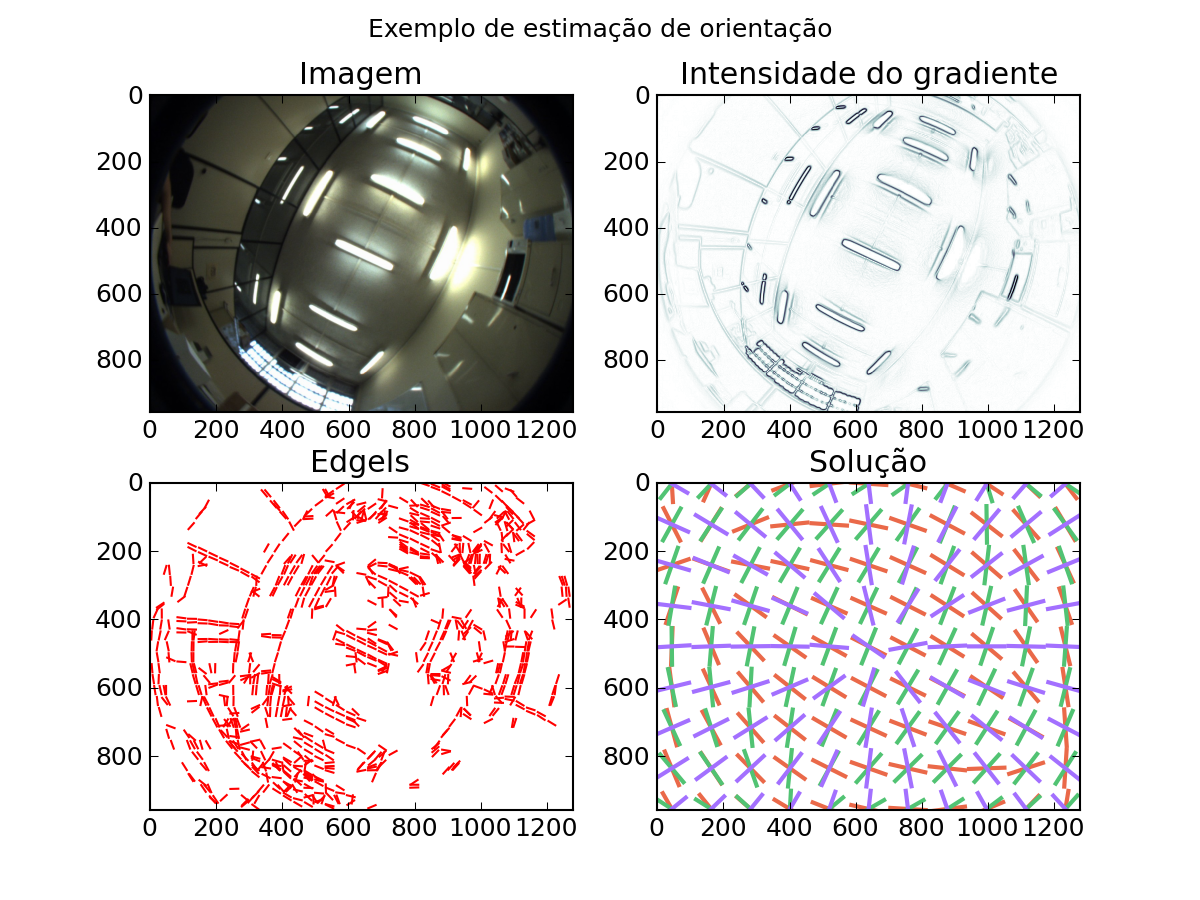
\includegraphics[height=14.2\baselineskip]{oriexfish6.png}}}
  \only<+>{\centerline{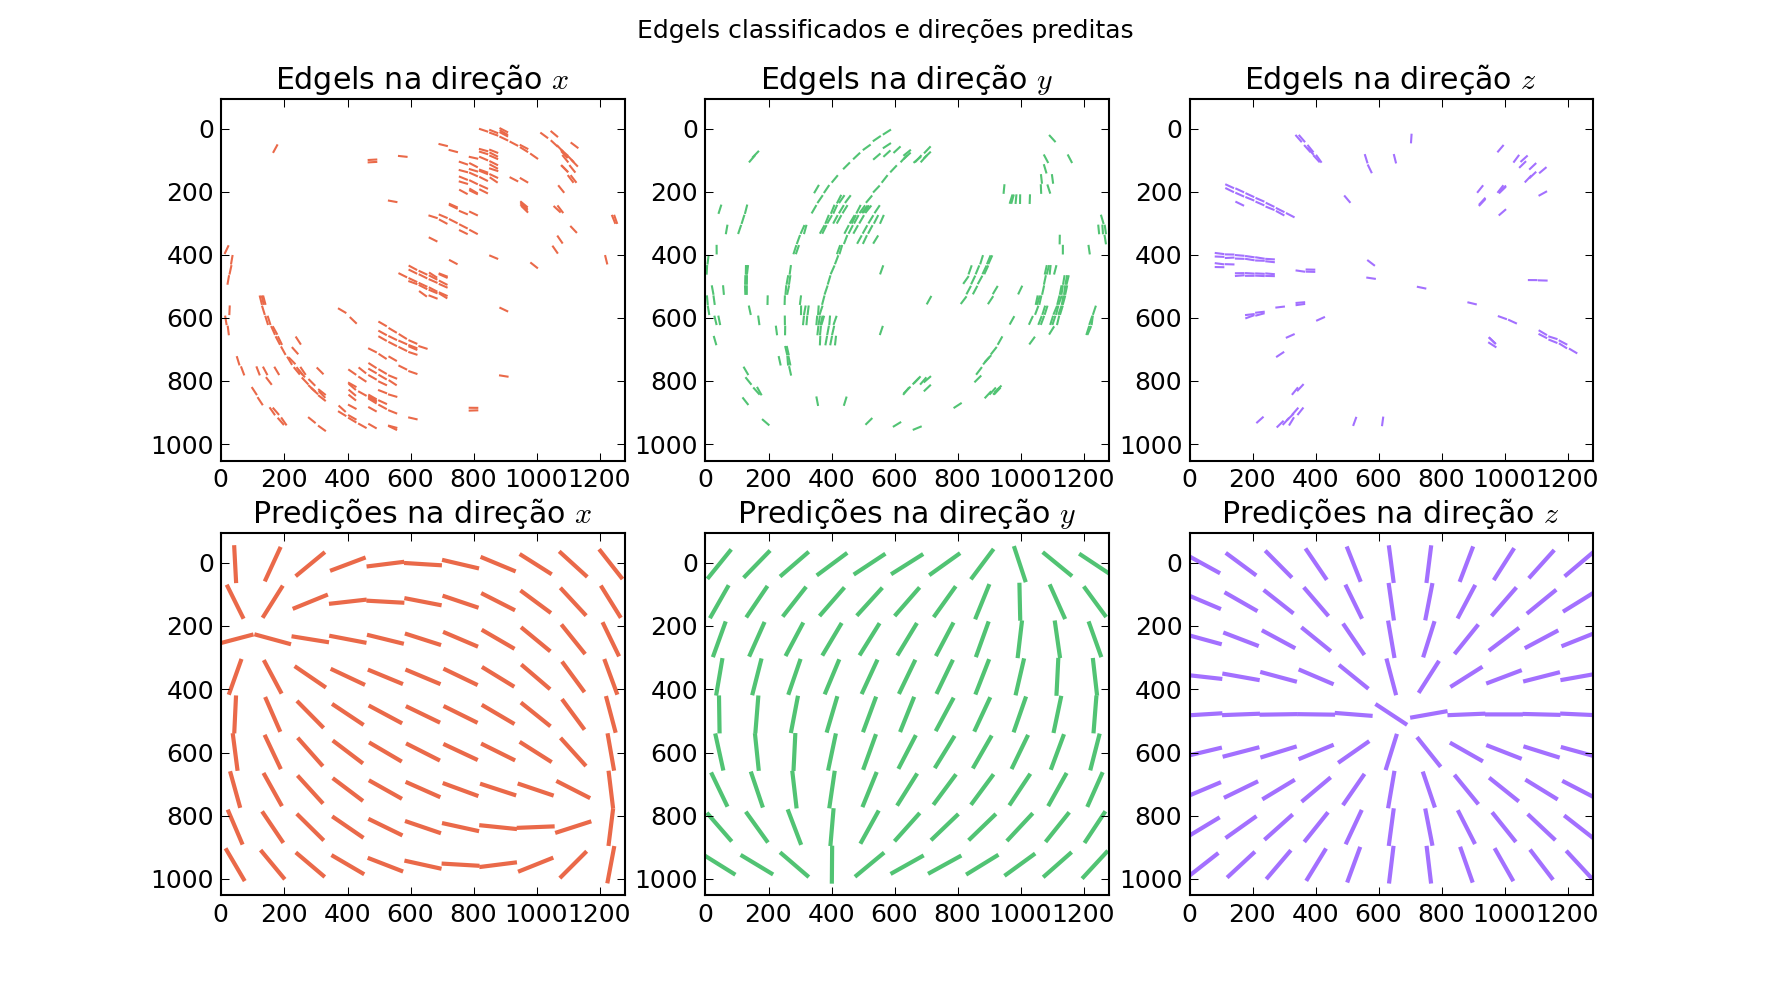
\includegraphics[height=14.2\baselineskip]{sep_fish6.png}}}
\end{frame}













%%%%%%%%%%%%%%%%%%%%%%%%%%%%%%
%%%%%%%%%%%%%%%%%%%%%%%%%%%%%%
\section[2--Corisco]{Detalhamento do Corisco}
%%
%%
\begin{frame}{Block diagram}
  \only<1>{\centerline{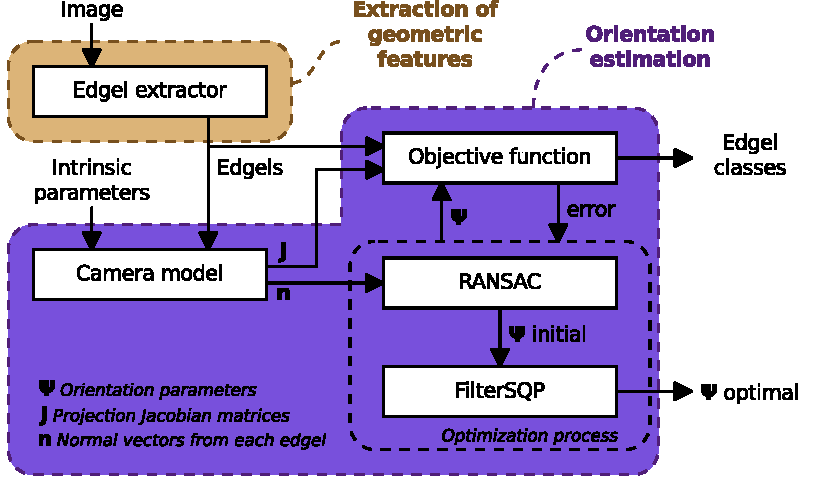
\includegraphics[height=12\baselineskip]{blocos_meta.pdf}}}
  \only<2>{\centerline{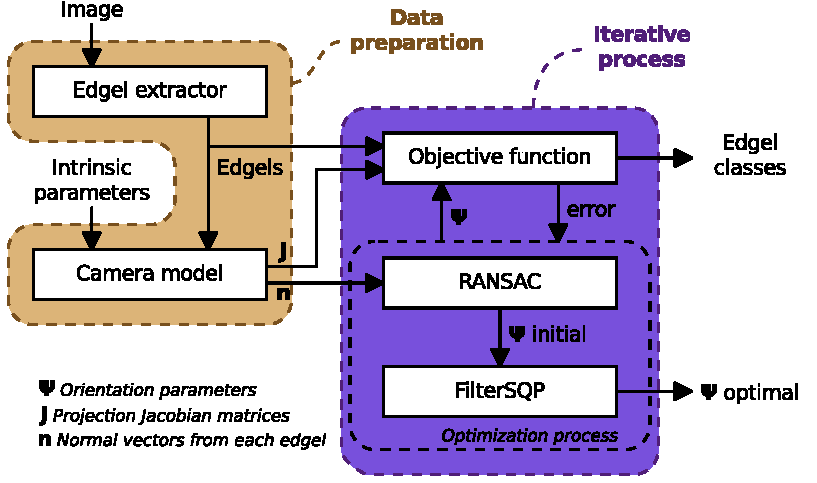
\includegraphics[height=12\baselineskip]{blocos_sep.pdf}}}
  \only<3>{\centerline{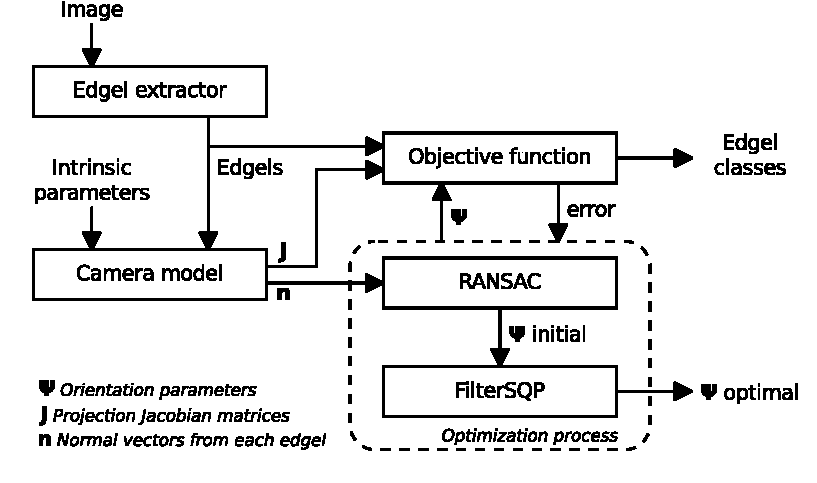
\includegraphics[height=12\baselineskip]{blocos.pdf}}}
\end{frame}







%%
%%
\begin{frame}{Extração de edgels}
  \centerline{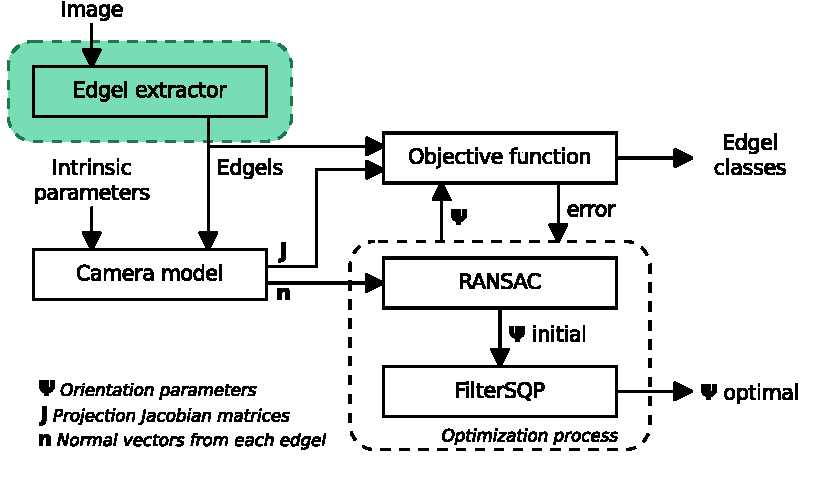
\includegraphics[height=12\baselineskip]{blocos_s1.pdf}}
  \begin{textblock*}{17mm}[1.0,0.0](\paperwidth-1px,1px)%
    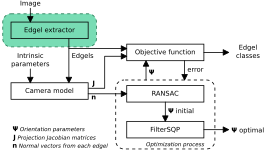
\includegraphics[width=17mm]{blocos_s1.png}%
  \end{textblock*}%
\end{frame}
\addtocounter{framenumber}{-1}

%%
%%
\begin{frame}{Extração de edgels}
  \begin{textblock*}{17mm}[1.0,0.0](\paperwidth-1px,1px)
    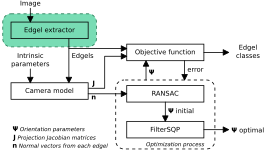
\includegraphics[width=17mm]{blocos_s1.png}
  \end{textblock*}
  \begin{itemize}
  \item Similar à detecção de bordas de Canny.\\
  \item Bordas são máximos locais na direção do gradiente.
  \end{itemize}
  \centerline{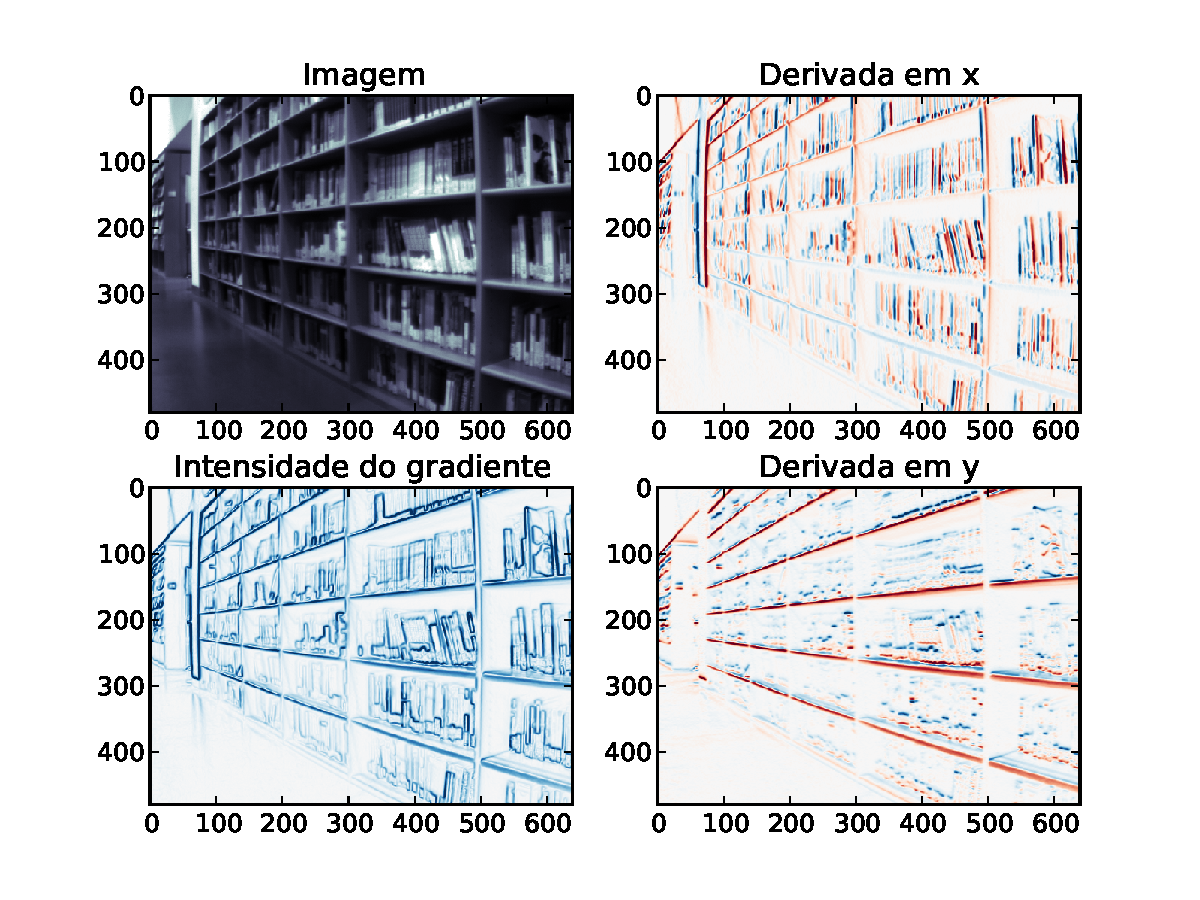
\includegraphics[height=12\baselineskip]{graddemo2.pdf}}
\end{frame}

%%
%%
\begin{frame}{Extração de edgels}
  \begin{textblock*}{17mm}[1.0,0.0](\paperwidth-1px,1px)
    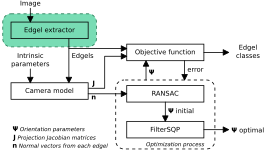
\includegraphics[width=17mm]{blocos_s1.png}
  \end{textblock*}
  Varredura da imagem sobre um conjunto de linhas e colunas que formam uma {\em
    máscara em forma de grade.}

  Cada borda encontrada produz um edgel. Sua direção deve ser aproximadamente
  ortogonal à da linha varrida.
  \centerline{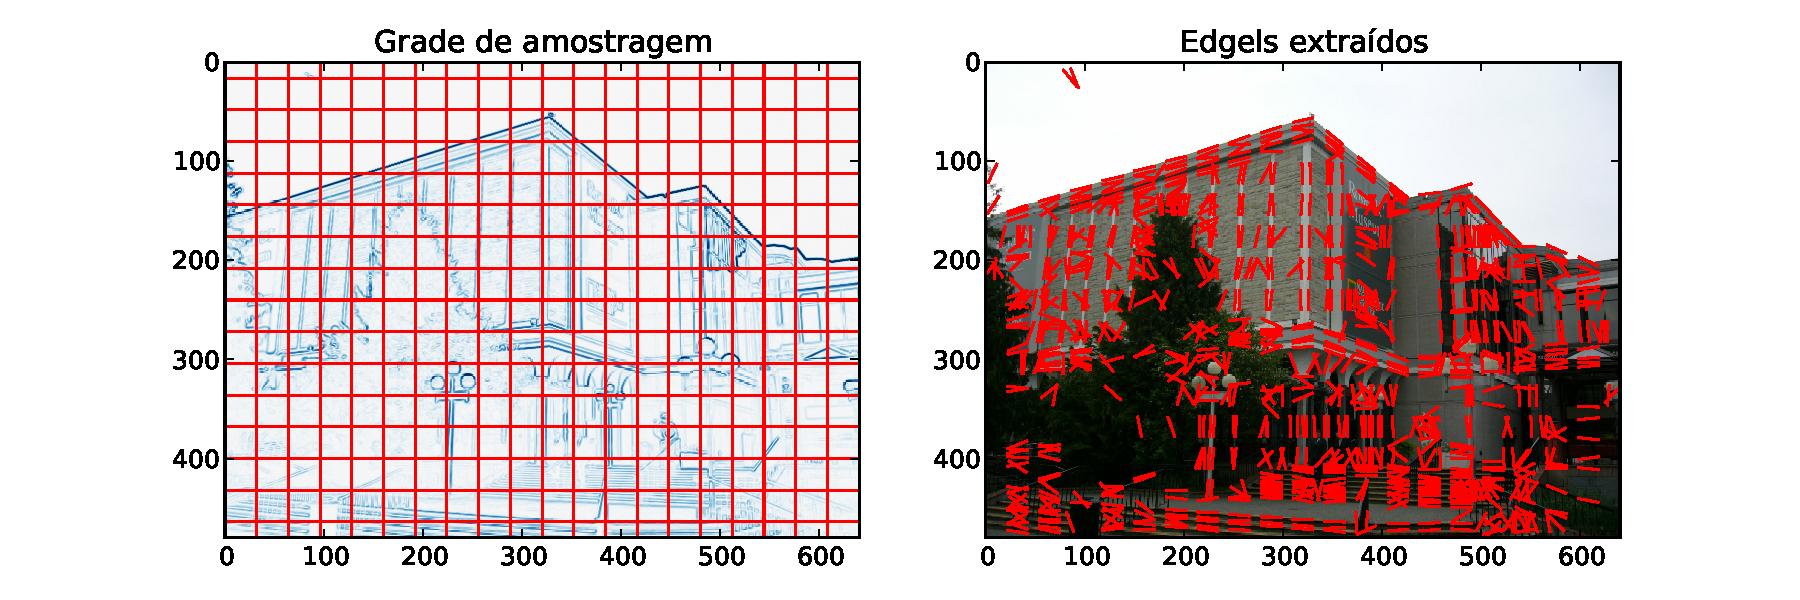
\includegraphics[height=8\baselineskip]{griddemo2.pdf}}

\end{frame}

%%
%%
% \begin{frame}{Extração de edgels}
%   \begin{textblock*}{17mm}[1.0,0.0](\paperwidth-1px,1px)
%     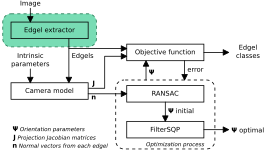
\includegraphics[width=17mm]{blocos_s1.png}
%   \end{textblock*}
%   Edgels são máximos locais da intensidade do gradiente, e aproximadamente ortogonais à linha varrida.
%   \centerline{
%     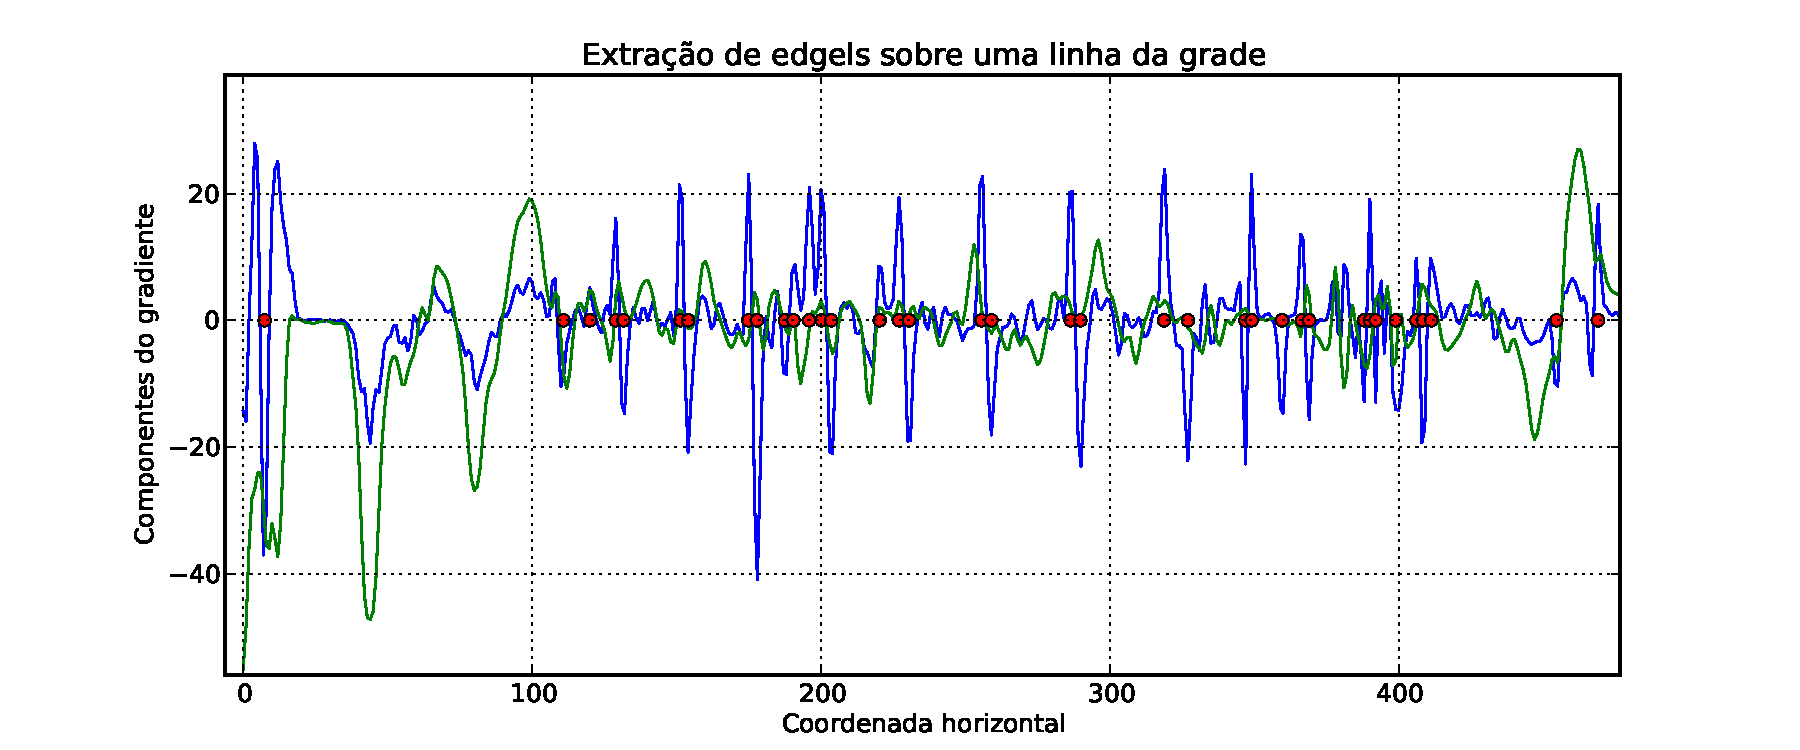
\includegraphics[height=10\baselineskip]{griddemo22.pdf}
%   }
% \end{frame}














%%
%%
\begin{frame}{Modelos de câmera}
  \only<1>{\centerline{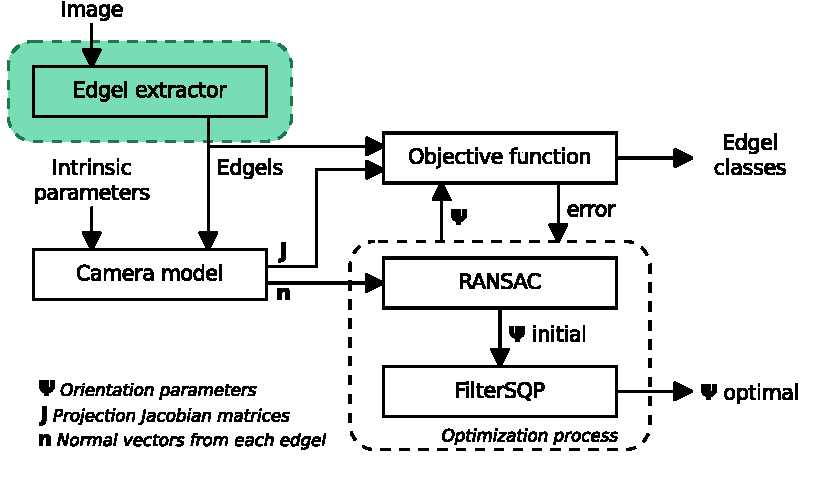
\includegraphics[height=12\baselineskip]{blocos_s1.pdf}}}
  \only<2>{\centerline{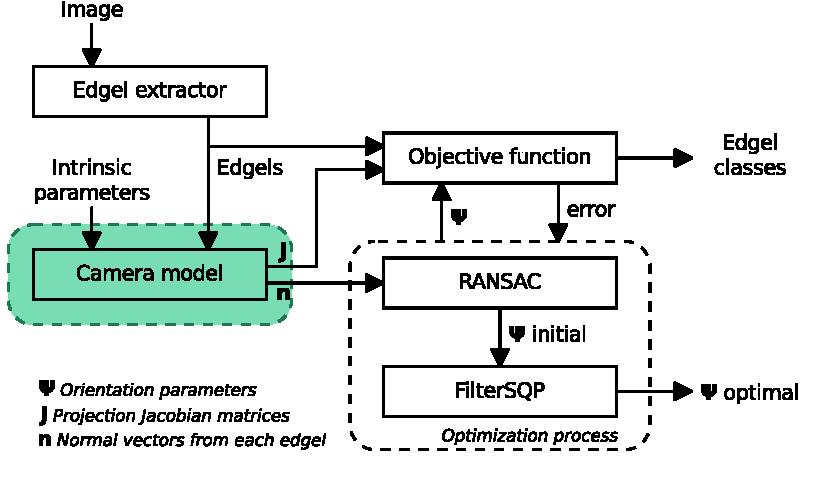
\includegraphics[height=12\baselineskip]{blocos_s2.pdf}}}
  \begin{textblock*}{17mm}[1.0,0.0](\paperwidth-1px,1px)
    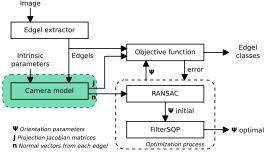
\includegraphics[width=17mm]{blocos_s2.png}
  \end{textblock*}
\end{frame}
\addtocounter{framenumber}{-1}


%% 
%%
\begin{frame}{Modelos de câmera}
  \begin{textblock*}{17mm}[1.0,0.0](\paperwidth-1px,1px)
    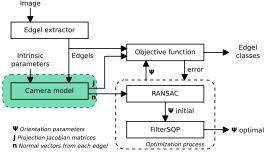
\includegraphics[width=17mm]{blocos_s2.png}
  \end{textblock*}
  Mapeamento bijetivo entre os pontos da imagem e direções ao redor do ponto
  focal da câmera.  
  \[\vq\rightleftharpoons\vp\]

  \begin{center}
    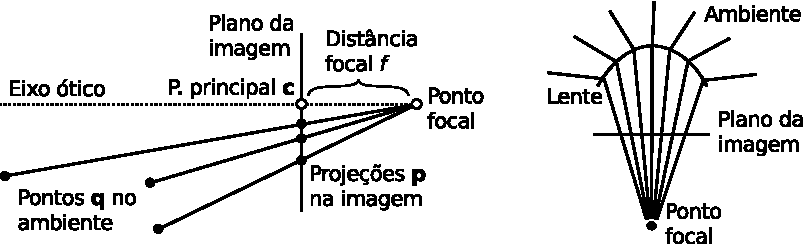
\includegraphics[height=6\baselineskip]{camera_model.pdf}   
  \end{center}
\end{frame}


%%
%%
\begin{frame}{Exemplos de modelos de câmera}
  \begin{textblock*}{17mm}[1.0,0.0](\paperwidth-1px,1px)
    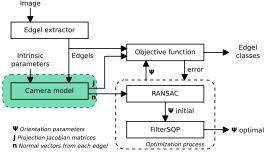
\includegraphics[width=17mm]{blocos_s2.png}
  \end{textblock*}
  Grande angular, olho-de-peixe, equiretangular.
  \centerline{
    \includegraphics[width=0.4\linewidth]{00000069.jpg}
    \includegraphics[width=0.4\linewidth]{fisheye.jpg}
  }
  \centerline{
    \includegraphics[width=0.8\linewidth]{00000029.jpg}
  }
\end{frame}


%%
%%
\begin{frame}{Equações de modelos de câmera}
  \begin{textblock*}{17mm}[1.0,0.0](\paperwidth-1px,1px)
    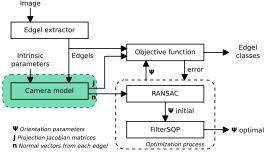
\includegraphics[width=17mm]{blocos_s2.png}
  \end{textblock*}
  \begin{center}
    \begin{tabular}{ll}
      Perspectiva & Equiretangular (lat-lon)\\
      \multicolumn{1}{c}{
        $\begin{array}{l}
        {\vp}^x = (\vq^x/\vq^z)f + \vc^x\\
        {\vp}^y = (\vq^y/\vq^z)f + \vc^y
      \end{array}$}
      &
      \multicolumn{1}{c}{
      $\begin{array}{l}
        \vp^x = f \tan^{-1}(\vq^z, \vq^x)\\
        \vp^y = f \sin^{-1}\left(\vq^y / |\vq| \right)
      \end{array}$}
      \\[\baselineskip]\\
      Harris (distorção radial) & Polar Equidistante (olho-de-peixe)\\
      \multicolumn{1}{c}{
      $\begin{array}{l}
        \label{eqn:raddist}
        g(x)=\frac{1}{\sqrt{1-2\kappa x^2}}\\
        \vp^x = {\vp^\prime}^x g(|\mathbf{\vp^\prime}|) + \vc^x\\
        \vp^y = {\vp^\prime}^y g(|\mathbf{\vp^\prime}|) + \vc^y
      \end{array}$}
      &
      \multicolumn{1}{c}{
      $\begin{array}{l}
        \varphi = \cos^{-1}\left(\vq^z /  |\vq| \right)\\
        \vp^x = \varphi\, \frac{\vq^x}{\sqrt{{\vq^x}^2+{\vq^y}^2}}f+\vc^x\\
        \vp^y = \varphi\, \frac{\vq^y}{\sqrt{{\vq^x}^2+{\vq^y}^2}}f+\vc^y
      \end{array}$}
    \end{tabular}
  \end{center}
\end{frame}

%%
%%
\begin{frame}{Projeção de um edgel}
  \begin{overprint}
  \begin{textblock*}{17mm}[1.0,0.0](\paperwidth-1px,1px)
    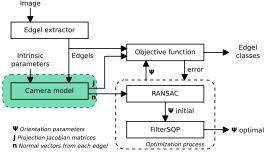
\includegraphics[width=17mm]{blocos_s2.png}
  \end{textblock*}
  Um ponto $\vq_n$ de uma reta na
  direção $\vr_k$ é projetado em $\vp_n$, produzindo um edgel com direção
  \begin{tabularx}{\linewidth}{XCR}
    & $\vv_{nk}\propto\vJ_n\vr_k$ & ~\uncover<2>{$\left(\vv\leftarrow(\vP,\vp)\right)$}
  \end{tabularx}
  
  A matriz Jacobiana da projeção $\vJ_n$ depende de $\vp_n$. A direção
  ortogonal a $\vv_n$ é denominada $\vu_n$.

  \centerline{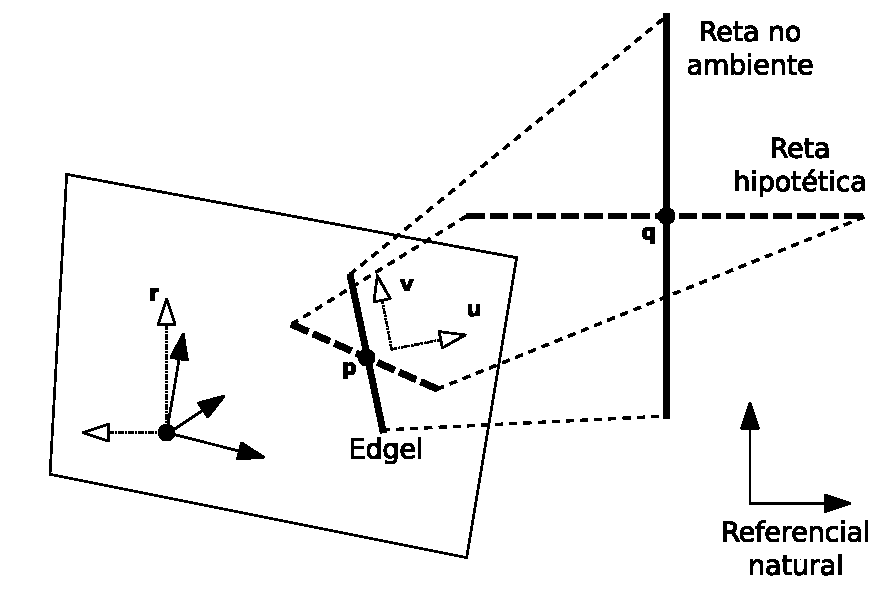
\includegraphics[height=8\baselineskip]{variaveis.pdf}}

\end{overprint}
\end{frame}


%%
%%
\begin{frame}{Normal de um edgel}
  \begin{textblock*}{17mm}[1.0,0.0](\paperwidth-1px,1px)
    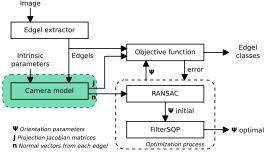
\includegraphics[width=17mm]{blocos_s2.png}
  \end{textblock*}

  Direção de um plano definido pelo ponto focal e por um edgel, ou uma reta
  correspondente no ambiente.
  \[
  \vn_k = \vu_k^x \vJ_k^x +  \vu_k^y \vJ_k^y
  \]

%  \centerline{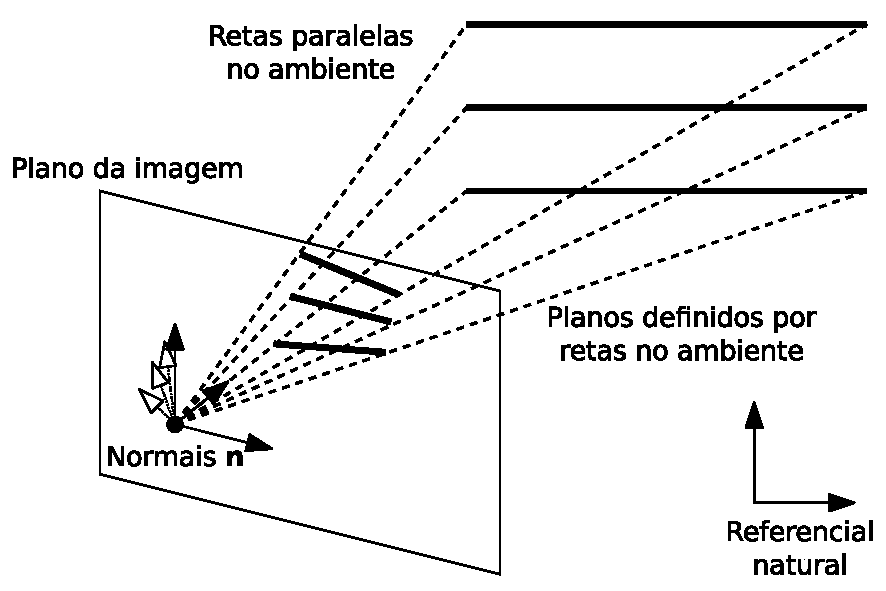
\includegraphics[height=8\baselineskip]{normal.pdf}}

\end{frame}














  






















%%
%%
\begin{frame}{Função objetivo}
  \only<1>{\centerline{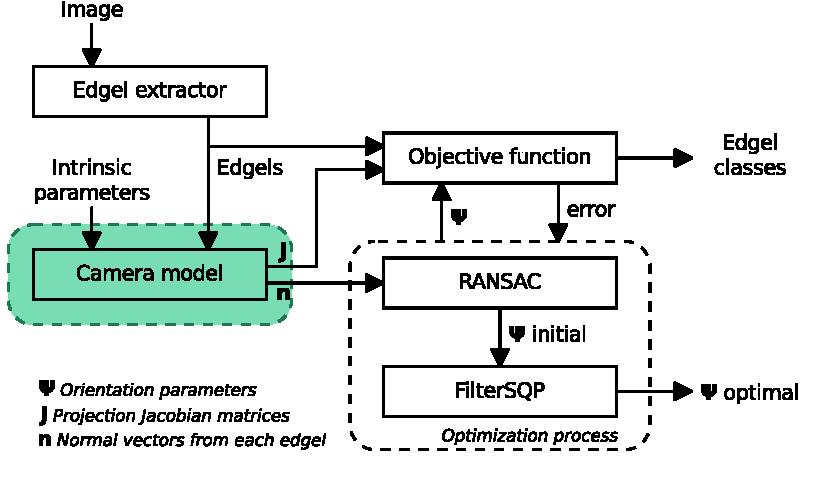
\includegraphics[height=12\baselineskip]{blocos_s2.pdf}}}
  \only<2>{\centerline{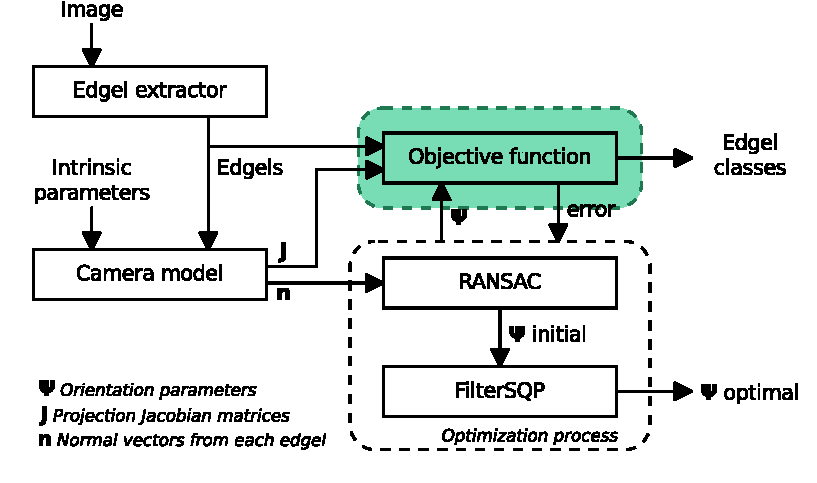
\includegraphics[height=12\baselineskip]{blocos_s3.pdf}}}
  \begin{textblock*}{17mm}[1.0,0.0](\paperwidth-1px,1px)
    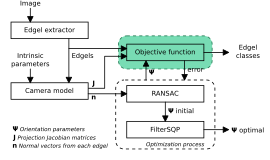
\includegraphics[width=17mm]{blocos_s3.png}
  \end{textblock*}
\end{frame}
\addtocounter{framenumber}{-1}

%%
%%
\begin{frame}{Função objetivo}
  \begin{textblock*}{17mm}[1.0,0.0](\paperwidth-1px,1px)
    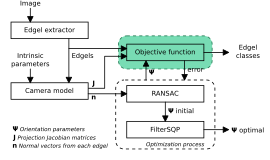
\includegraphics[width=17mm]{blocos_s3.png}
  \end{textblock*}

  A função objetivo é o cerne do método.\\
  \begin{itemize}
  \item Independe da técnica de extração.
  \item Determina o resultado.
  \item Conduz a escolha do algoritmo de otimização.
  \end{itemize}
  
  A expressão tem a forma de uma soma de erros obtidos de cada observação.
  \[
  y_n = x_n - \hat{x}_n(\vP)
  \]\[
  F(\vP) = \sum_n (y_n)^2
  \]
\end{frame}

\begin{frame}{Matriz de rotação}
  \begin{textblock*}{17mm}[1.0,0.0](\paperwidth-1px,1px)
    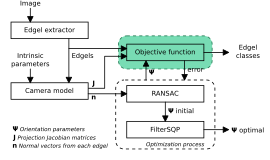
\includegraphics[width=17mm]{blocos_s3.png}
  \end{textblock*}

  O cálculo das predições começa com o cálculo das direções do referencial
  natural $\vr_k$ em função de $\vP$.
  
  O \corisco trabalha com quaternions.
  \[
  \vP = (\Pa, \Pb, \Pc, \Pd) \qquad |\vP|=1
  \]
  
  Para uma orientação $\vP$ qualquer temos
  \[
  \mathbf{R}(\vP) =
  \left[
    \begin{array}{l}
      \vr_x\;
      \vr_y\;
      \vr_z
    \end{array}
  \right]^T = 
  \]
  \[\hspace{-.8em}\footnotesize
  \left[
    \begin{array}{ccc}
      \Pa^2+\Pb^2-\Pc^2-\Pd^2 &2\Pb\Pc+2\Pa\Pd & 2\Pb\Pd-2\Pa\Pc\\
      2\Pb\Pc-2\Pa\Pd& \Pa^2-\Pb^2+\Pc^2-\Pd^2&2\Pc\Pd+2\Pa\Pb\\
      2\Pb\Pd+2\Pa\Pc& 2\Pc\Pd-2\Pa\Pb& \Pa^2-\Pb^2-\Pc^2+\Pd^2\\
    \end{array}
  \right]
  \]
\end{frame}

%%
%%
\begin{frame}{Resíduo de um edgel}
  \begin{textblock*}{17mm}[1.0,0.0](\paperwidth-1px,1px)
    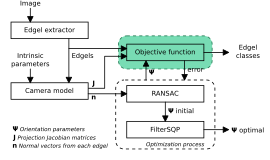
\includegraphics[width=17mm]{blocos_s3.png}
  \end{textblock*}

  Dados os $\vr_k$, calculam-se as direções preditas $\vv_{nk}$ utilizando $\vJ_k$.
  \[
  \vP \rightarrow \vr_k \rightarrow \vv_{nk}
  \]
  \[
  \vv_{nk}\propto\vJ_n\vr_k
  \]
  
  O resíduo é obtido entre:\\
  \begin{itemize}
  \item $\vv_n$ (ou $\vu_n$) medidos da imagem.
  \item $\vv_{nk}$ preditas a partir de $\vP$ e $\vp_n$.
  \end{itemize}

  \begin{center}
    \begin{tabularx}{\textwidth}{XX}
      Métodos anteriores: & \corisco:\\
      \multicolumn{1}{l}{
        \quad$\angle\vv = \arctan(\vv^x, \vv^y)$}
      &
      \multicolumn{1}{l}{
        \quad$\vu_n\vv_{nk}$
      }\\
      \multicolumn{1}{l}{
        \quad$\angle\vv_n - \angle\vv_{nk}$}&\\
    \end{tabularx}
  \end{center}
\end{frame}



%%
%%
\begin{frame}{Técnicas de estimação}
  \begin{textblock*}{17mm}[1.0,0.0](\paperwidth-1px,1px)
    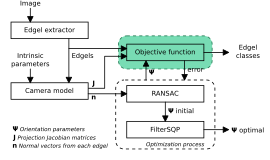
\includegraphics[width=17mm]{blocos_s3.png}
  \end{textblock*}
  Comparação de técnicas já utilizadas com edgels:

  {\footnotesize
    \begin{tabularx}{\textwidth}{lCCC}
      \toprule
      & MAP & EM & M-estimação\\
      \hline
      Modelos & Probabilístico & Probabilístico & $\rho(x)$ \\
      Classes & 4 & 4 & 3\\ 
      Classificação & $\times$ & Iterativa & Direta\\
      % Etapas & 1 & 2 & 1 \\ 
      \bottomrule
    \end{tabularx}
  }
  
  \hspace{-0.25\baselineskip}\centerline{
    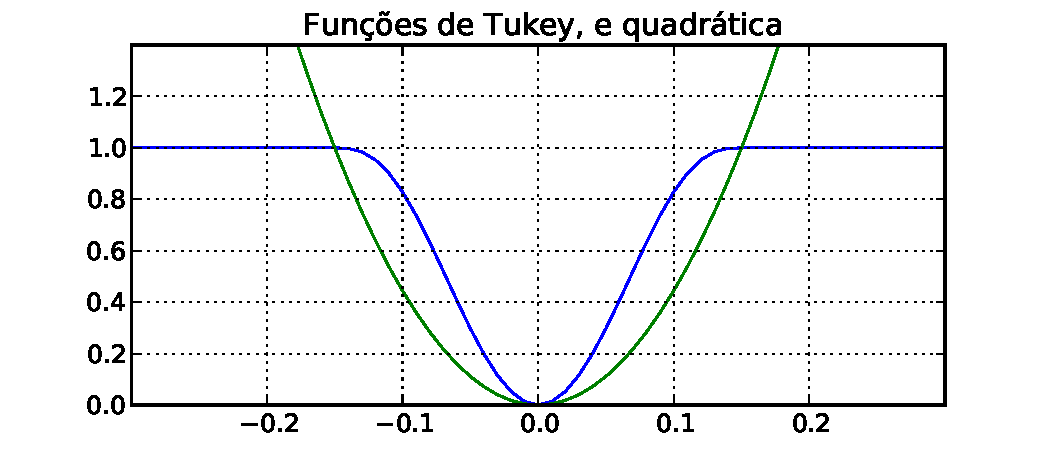
\includegraphics[height=7\baselineskip]{tukey.pdf}
  }
\end{frame}





%%
%%
\begin{frame}{Expressão da função objetivo}
  \begin{textblock*}{17mm}[1.0,0.0](\paperwidth-1px,1px)
    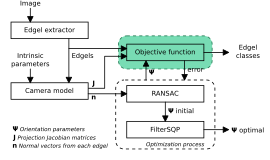
\includegraphics[width=17mm]{blocos_s3.png}
  \end{textblock*}

  Estimador MAP~(\cite{Coughlan2003}):
  \[
  F(\vP) =
  -\sum_n\log\left(
    \sum_k  p(c_n=k)p(\angle\vv_n|\vP,\vp_n,c_n=k)
  \right)
  \]
  
  Estimador EM~(\cite{Schindler2004}):
  \[F(\vP) = -\sum_n \sum_k p(c_n=k) \log\left(
    p(\angle\vv_n|\vP,\vp_n,c_n=k)
  \right)\]
  \[F(\vP) = \sum_n \sum_k p(c_n=k) \left(\angle\vv_n-\angle\vv_{nk}\right)^2\]

  \corisco:
  \[
  F(\vP) = \sum_n \min_k \rho(\vu_n \vv_{nk})
  \]

  % \begin{textblock*}{\textwidth}[0.5,0.0](0.5\paperwidth,6\baselineskip)
  %   ~\only<2>{
  %     \begin{tcolorbox}[enlarge left by=-5mm,width=\linewidth+10mm,colback=green!12,colframe=green]
  %       \[F(\vP) = -\sum_n \sum_k p(c_n=k) \log\left(p(\angle\vv_n|\vP,\vp_n,c_n=k)\right)\]
  %     \end{tcolorbox}
  %   }
  % \end{textblock*}
  \begin{textblock*}{1.0\textwidth}[0.5,0.0](0.5\paperwidth,7.42\baselineskip)
    \only<2>{
      \begin{tcolorbox}[enlarge left by=-5mm,width=\linewidth+10mm,colback=green!12,colframe=green]
        ~\\~\\~
      \end{tcolorbox}
    }
  \end{textblock*}
  \begin{textblock*}{1.1\textwidth}[0.5,0.0](0.5\paperwidth,8.58\baselineskip)
    \only<2>{
        \[F(\vP) = -\sum_n \sum_k p(c_n=k) \log\left(
          p(\angle\vv_n|\vP, \vp_n, c_n=k)
        \right)\]
    }
  \end{textblock*}
  \begin{textblock*}{\textwidth}[0.5,0.0](0.5\paperwidth,9.8\baselineskip)
    \only<3>{
      \begin{tcolorbox}[enlarge left by=-5mm,width=\linewidth+10mm,colback=green!12,colframe=green]
        \[F(\vP) = \sum_n \sum_k p(c_n=k) \left(\angle\vv_n-\angle\vv_{nk}\right)^2\]
      \end{tcolorbox}
    }
  \end{textblock*}
  \begin{textblock*}{\textwidth}[0.5,0.0](0.5\paperwidth,12.65\baselineskip)
    \only<4>{
      \begin{tcolorbox}[enlarge left by=-5mm,width=\linewidth+10mm,colback=red!12,colframe=red]
        \hspace{-0.5mm}\corisco:
        \[
        F(\vP) = \sum_n \min_k \rho(\vu_n \vv_{nk})
        \]
      \end{tcolorbox}
    }
  \end{textblock*}


  
\end{frame}

























%%
%%
\begin{frame}{Otimização}
  \only<1>{\centerline{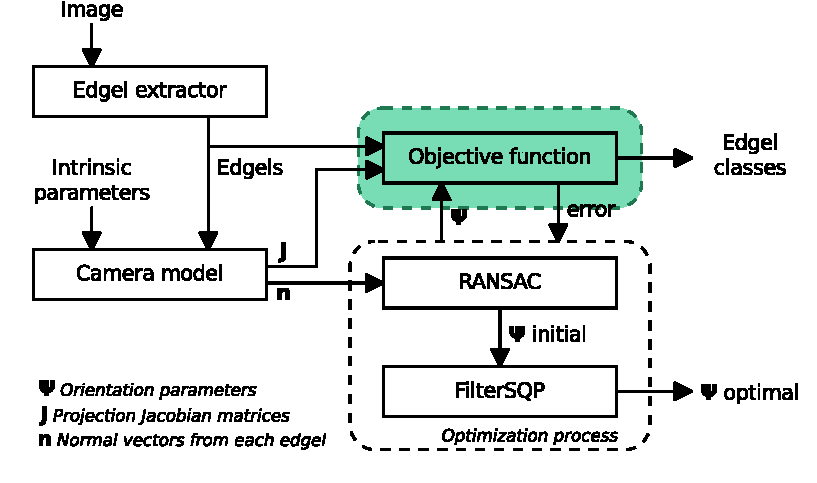
\includegraphics[height=12\baselineskip]{blocos_s3.pdf}}}
  \only<2>{\centerline{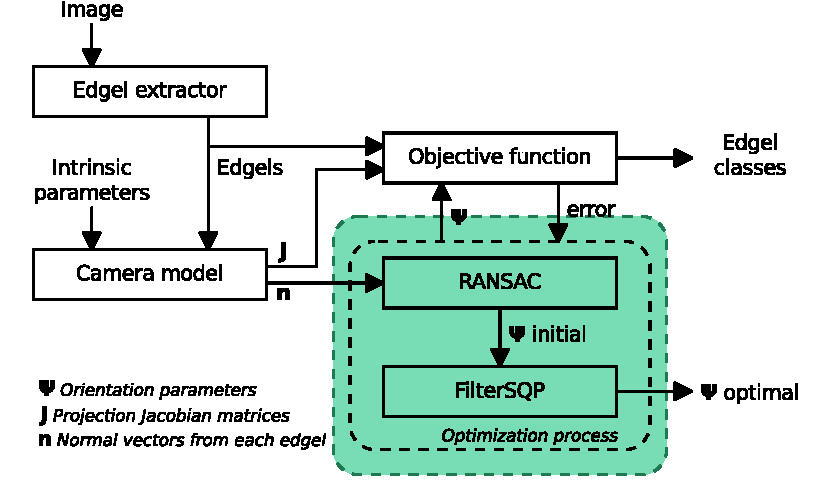
\includegraphics[height=12\baselineskip]{blocos_s4.pdf}}}
  \begin{textblock*}{17mm}[1.0,0.0](\paperwidth-1px,1px)
    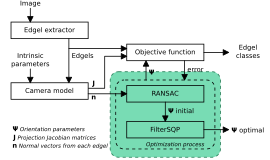
\includegraphics[width=17mm]{blocos_s4.png}
  \end{textblock*}
\end{frame}
\addtocounter{framenumber}{-1}

%%
%%
\begin{frame}{Otimização}{}
  {\bf Primeiro passo:} RANSAC, busca estocástica guiada pelos
  dados. Inerentemente ineficiente e impreciso.

  \uncover<2->{$\rightarrow \vP$ inicial}

  {\bf Segundo passo:} FilterSQP, otimização contínua, mais eficiente e
  precisa do que o RANSAC.
  
  \uncover<3>{$\rightarrow \vP$ final}

\end{frame}


%%
%%
\begin{frame}{RANSAC}
  \begin{textblock*}{17mm}[1.0,0.0](\paperwidth-1px,1px)
    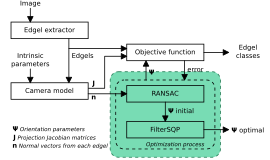
\includegraphics[width=17mm]{blocos_s4.png}
  \end{textblock*}

  Triplas de observações são selecionadas ao acaso. De  cada tripla calcula-se um $\vP$ hipotético, utilizando
  $\vn_k$.
  
  O $\vP$ de menor $F(\vP)$ é retido como estimativa inicial.
  \centerline{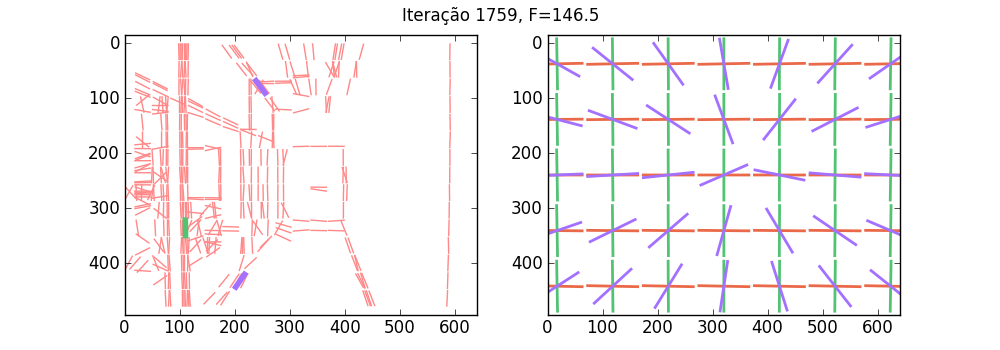
\includegraphics[height=8\baselineskip]{rdemo0014.png}}
\end{frame}


%%
%%
\begin{frame}{FilterSQP}
  \begin{textblock*}{17mm}[1.0,0.0](\paperwidth-1px,1px)
    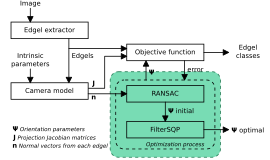
\includegraphics[width=17mm]{blocos_s4.png}
  \end{textblock*}
  Minimizar $F(\vP)$ sobre as 4D e restrito a
  $|\vP|=1$.

  \begin{tabular}{rcl}
    {\em Programa não-linear} & $\rightarrow$ & \parbox{12em}{\centering{\bf SQP:} Sequential Quadratic Programming}
  \end{tabular}
  
  O FilterSQP (\cite{Fletcher2002}) dispensa funções de penalidade.
  \centerline{
    \includegraphics[height=9\baselineskip]{sqp_traj.png}
  }
\end{frame}

\begin{frame}{Derivada}
  \begin{textblock*}{17mm}[1.0,0.0](\paperwidth-1px,1px)
    \includegraphics[width=17mm]{blocos_s4.png}
  \end{textblock*}
  No \corisco as derivadas em $\vP$ são calculadas através de fórmulas fechadas.
  \[
  \frac{\partial F}{\partial\Pa}(\vP) = \sum_{nk}K_{nk}\,\rho^\prime(\vu_n\vv_{nk})
  \left(u_n^x\frac{\partial\vv_{nk}^x}{\partial\Pa} + u_n^y\frac{\partial\vv_{nk}^y}{\partial\Pa}\right)
  \]

  As derivadas das direções $\vr_k$ são triviais:
    \begin{eqnarray*}
      \frac{\partial \vr^x}{\partial \Pa} &=& 2( \Pa, \Pd,-\Pc)\\
      \frac{\partial \vr^x}{\partial \Pb} &=& 2( \Pb, \Pc, \Pd)\\
      &\cdots&
    \end{eqnarray*}
  
\end{frame}

















%%%%%%%%%%%%%%%%%%%%%%%%%%%%%%
%%%%%%%%%%%%%%%%%%%%%%%%%%%%%%
\section[5--Experimentos]{Experimentos}

%%
%%
\begin{frame}{Experimentos}
  Foram realizados 3 experimentos que permitem avaliar o desempenho do
  \corisco.

  Cada experimento utilizou um conjunto de imagens, e um método diferente para
  obter orientações de referência.

  O erro observado é o deslocamento em graus da ``rotação residual'' entre
  cada estimativa e referência.

  O \corisco foi executado variando-se\\
  \begin{itemize}
  \item o tamanho da grade,
  \item e o número de iterações do RANSAC.
  \end{itemize}
\end{frame}

%% 
%%
\begin{frame}{YorkUrbanDB}{}
  {\bf Imagens:} 101 imagens de ambientes antrópicos.

  {\bf Modelo:} Perspectiva.

  {\bf Referência:} Método semi-automático baseado em retas.

  {\bf Comparação:} Métodos testados por \cite{Denis2008}.

  Parâmetros do modelo, orientações de referência e estatísticas de
  desempenho fornecidos pelos autores.

\end{frame}

\begin{frame}{YorkUrbanDB}
\begin{center}
\begin{tabular}{cc}
  \includegraphics[width=0.45\textwidth]{P1020177.jpg}&
  \includegraphics[width=0.45\textwidth]{P1020819.jpg}\\
  \includegraphics[width=0.45\textwidth]{P1040811.jpg}&
  \includegraphics[width=0.45\textwidth]{P1080092.jpg}
\end{tabular}
\end{center}
\end{frame}

%%
%%

\begin{frame}{YorkUrbanDB}
\begin{overprint}
\def\animrow{}
\only<2->{\def\animrow{\rowcolor[rgb]{1.0,0.5,0.5}}}
\def\animcc{}
\only<3->{\def\animcc{\cellcolor[rgb]{0.47,0.86,0.70}}}
\def\animccc{}
\only<4>{\def\animccc{\cellcolor[rgb]{0.47,0.86,0.70}}}
\footnotesize
\begin{textblock*}{\paperwidth}[0,0.5](0mm,0.5\paperheight)
\begin{center}
\begin{tabular}{l|r|cc|ccc}
Method           & Time & \multicolumn{5}{c}{Error} \\
\cline{3-7}
           & \multicolumn{1}{c|}{[s]} & Mean & $\sigma$& 1/4 & Median  & 3/4 \\
\hline
EM Newton        & $27+?$ & $4.00^\circ$ & $1.00^\circ$
                 & \animccc $1.15^\circ$ & \animccc $2.61^\circ$ & \animccc $4.10^\circ$\\
MAP Quasi-Newton & $6+?$  & $4.00^\circ$ & $1.00^\circ$
                 & $1.32^\circ$ & $2.39^\circ$ & $4.07^\circ$ \\
EM Quasi-Newton  & \animcc $1+?$  & $9.00^\circ$ & $1.00^\circ$
                 & $4.04^\circ$ & $6.21^\circ$ & $10.33^\circ$\\

J-linkage        & $1.13$  & $8.23^\circ$ & $13.76^\circ$
                 & $1.14^\circ$ & $2.36^\circ$ & $4.44^\circ$\\
\hline
{\em Corisco} $C_r=10^4\; C_g=1$
                 & $47.20$   & $1.51^\circ$ & $3.26^\circ$
                 & $0.69^\circ$&$1.09^\circ$&$1.51^\circ$\\
{\em Corisco} $C_r=10^4\; C_g=4$
                 & $16.68$   & $1.71^\circ$ & $3.35^\circ$
                 & $0.72^\circ$&$1.14^\circ$&$1.64^\circ$\\
{\em Corisco} $C_r=10^4\; C_g=32$
                 & $7.57$   & $2.43^\circ$ & $4.03^\circ$
                 & $0.97^\circ$&$1.54^\circ$&$2.42^\circ$\\
\hline
{\em Corisco} $C_r=10^3\; C_g=1$
                 & $8.12$   & $1.70^\circ$ & $3.22^\circ$
                 & $0.70^\circ$&$1.11^\circ$&$1.77^\circ$\\
{\em Corisco} $C_r=10^3\; C_g=4$
                 & $2.50$   & $2.02^\circ$ & $3.86^\circ$
                 & $0.81^\circ$&$1.24^\circ$&$1.80^\circ$\\
\animrow{\em Corisco} $C_r=10^3\; C_g=32$
                 & $0.99$   & $2.44^\circ$ & $3.54^\circ$
                 & $1.00^\circ$&$1.68^\circ$&$2.64^\circ$\\
\hline
{\em Corisco} $C_r=200\; C_g=1$
                 & $5.34$   & $2.08^\circ$ & $3.38^\circ$
                 & $0.72^\circ$&$1.22^\circ$&$1.78^\circ$\\
{\em Corisco} $C_r=200\; C_g=4$
                 & $1.89$   & $3.27^\circ$ & $6.38^\circ$
                 & $0.85^\circ$&$1.34^\circ$&$2.35^\circ$\\
{\em Corisco} $C_r=200\; C_g=32$
                 & $0.45$   & $3.29^\circ$ & $4.99^\circ$
                 & $0.99^\circ$&$1.72^\circ$&$3.46^\circ$\\
\end{tabular}
\end{center}
\end{textblock*}
\end{overprint}
\end{frame}
















%%
%%
\begin{frame}{ApaSt}{}
  {\bf Imagens:} 24+24 imagens de edifícios.

  {\bf Modelo:} Perspectiva com distorção radial (Harris).

  {\bf Referência:} {\em Bundler}.

  \begin{center}
    \includegraphics[height=6\baselineskip]{apast01.jpg}\quad
    \includegraphics[height=6\baselineskip]{apast02.jpg}
  \end{center}
\end{frame}


%%
%%
\begin{frame}{ApaSt}
  O {\em Bundler} (\cite{Snavely2006}) foi utilizado para obter as orientações
  de referência e os parâmetros intrínsecos.

  Método multi-ocular baseado em pontos.

  \begin{center}
    \fbox{\includegraphics[width=0.45\textwidth]{meshlab01.png}}
    \fbox{\includegraphics[width=0.45\textwidth]{meshlab02.png}}
  \end{center}
\end{frame}



%%
%%
\begin{frame}{ApaSt}
  \only<+>{\centerline{\includegraphics[height=11\baselineskip]{ava-apa10000.pdf}}}
  \only<+>{\centerline{\includegraphics[height=11\baselineskip]{ava-apa1000.pdf}}}
\end{frame}






%%
%%
\begin{frame}{StreetView}{}
  {\bf Imagens:} 250 imagens de um ambiente urbano.

  {\bf Modelo:} Projeção equiretangular.

  {\bf Referência:} Sensores físicos (IMU).
  \centerline{\includegraphics[height=10\baselineskip]{equi.png}}
\end{frame}

%%
%%
\begin{frame}{StreetView}
  Erro $\simeq 1^\circ$, tempo $\simeq 17$s.

\begin{center}
    \includegraphics[height=12\baselineskip]{street_fit.pdf}
  \end{center}
\end{frame}
  

%%
%%
\begin{frame}{Conclusão}
  O \corisco constitui um método com grande potencial para aplicação imediata.\\
  \begin{itemize}
  \item Implementação relativamente simples.
  \item Grande robustez (distorções, RANSAC).
  \item Bom desempenho.
  \end{itemize}
  
  Demonstrou-se as vantagens do uso da máscara em forma de grade, e da
  M-estimação.

  Também foi demonstrado como  utilizar o FilterSQP para trabalhar naturalmente
  com quaternions.
\end{frame}  

\begin{frame}{Trabalhos futuros}
  \begin{itemize}
  \item Controle automático dos parâmetros.
  \item Reconstrução multi-ocular e monocular.
  \item Utilizar filtros direcionais para medir o erro angular.
  \item Utilizar a máscara de grade em outros problemas.
  \item Estimar orientação e calibração, e extrair curvas em um processo
    unificado. (MRF?)
  \end{itemize}
\end{frame}



\begin{frame}{Fim}
\begin{minipage}{10em}
  Obrigado!
\end{minipage}
\begin{minipage}{10em}
  \centerline{\includegraphics[height=11\baselineskip]{myrobot.jpg}}
\end{minipage}

\vfill
\begin{block}{Financiamento}
  Obrigado à Capes, CNPq e USP pelo suporte financeiro.
\end{block}
\end{frame}



%%%%%%%%%%%%%%%%%%%%%%%%%%%%%%
%%%%%%%%%%%%%%%%%%%%%%%%%%%%%%
\appendix
\newcounter{finalframe}
\setcounter{finalframe}{\value{framenumber}}


\begin{frame}{Publicações}
  \begin{itemize}
  \item {\em Speeding up probabilistic inference of camera orientation by function approximation and grid masking}, \cite{Werneck2011}
  \item {\em Mapping with monocular vision in two dimensions}, \cite{Werneck2010b}
  \item {\em Medição de distância e altura de bordas horizontais com visão monocular linear para robôs móveis}, \cite{Werneck2009}
  \end{itemize}
\end{frame}

\begin{frame}[allowframebreaks]
\section*{Referências}
\centerline{ \bf Referências Bibliográficas}
\vspace{-1\baselineskip}
\footnotesize
 \bibliographystyle{plainnat}
 \bibliography{defesa}
\end{frame}




%%
%%
\begin{frame}{Teste de calibração}
 Estimação da distância focal com a mesma $F(\vP)$.
\centerline{
    \includegraphics[height=12\baselineskip]{edgel_cali.pdf}
  }
\end{frame}







\end{document}






%%% Local Variables:
%%% coding: utf-8
%%% default-justification: left
%%% fill-column: 79
%%% End:



